% Chapter 1

\chapter{An on-line implementation for the Odroid-XU developer board}

\lhead{Chapter 5. \emph{An on-line implementation}} % This is for the header on each page - perhaps a shortened title

%----------------------------------------------------------------------------------------
The last contribution of this thesis is a real-time implementation of our gesture recognition approach, ready to be used on an embedded device and which could be suitable for real-world application. To this aim, we need to modify and improve the classification module of our gesture recognition algorithm, replacing the simple linear SVM classifier with a more complex Structural SVM implementation, designed to take a stream of frames as input, and choose the Odroid-XU developer board as our target plaform. To make our implementation capable of running in real-time, we also have to exploit several optimization techniques.

\section{Splitting trajectories}
In the previous chapter, we classified frame sequences containing a gesture using a linear and power-normalized SVM classifier. In particular, we extracted trajectories with fixed length $L=30$ from the frame sequence, we then applied a standard BoW approach, and the output of the BoW was our final feature vector, with fixed size and ready to be classified with a standard SVM classifier. Note that in this case the input of the BoW was a feature vector describing the whole trajectory, therefore the SVM classifier was given a description of the entire frame sequence as input. That has been, so far, our way of taking time into account. Unfortunately, this only works when we have a frame sequence containing exactly one gesture, that is, when we know where a gesture starts and ends.

Now, we consider a more complex scenario: we have a stream of frames, whose length is unknown, that can contain a variable number of gestures, and we have to classify each frame as if it contains a gesture (and which gesture) or not. This is basically a \textit{label sequence learning} problem, with one more class than the ones we were used to, the \textit{non-gesture} one.

We start observing that our trajectory descriptors can be thought as a concatenation of single-point descriptors. Formally, let's consider a trajectory $T_i$ starting at frame $t_i$ and ending at frame $t_i+L-1$: we can express $T_i$ as $\left[ P_{t_i}^i, P_{t_{i+1}}^i, ..., P_{t_i+L-1}^i \right]$, where $P_{j}^i$ is the point of trajectory $T_i$ at frame $j$.  If we denote $D(T_i)$ the descriptor of trajectory $T_i$, then $D(T_i)$ can be expressed as the concatenation of $d(P_{t_i}^i), d(P_{t_{i+1}}^i), ..., d( P_{t_i+L-1}^i)$, where $d(P_{j}^i)$ is a descriptor computed around $P_j^i$, at frame $j$. 

Let's now consider a single frame $j$ of a frame stream, and suppose $ \{ T_1, T_2, ..., T_n\}$ are the trajectories crossing this frame. In this on-line version, we build a BoW histogram on each frame, being the input of the BoW clustering the set of descriptors of the trajectory points crossing the frame, i.e. $\{ d(P_{j}^1),  d(P_{j}^2), ...,  d(P_{j}^n) \}$.  Therefore, the corresponding BoW histogram won't represent a collection of trajectories anymore, but a collection of points, each one belonging to a different trajectory, and all related to the same frame.

Shortly, in the previous chapter the temporal dimension was encoded directly into the BoW input, now this will be up to the sequence classifier.


\section{Classification}
 In Section \ref{svmhmm} we have already described how a Struct SVM classifier can be used for label sequence learning. Now, we exploit the Structural SVM implementation by Altun \etal using this modified version of our feature vectors.

 We modify the source code provided by Joachims \cite{joachims} in order to include higher order label-label and label-features interactions, so that the generic 
$\Psi(\mathbf{x},\mathbf{y})$ takes the following form:

\begin{equation}
\Psi_{\epsilon,\tau}(\mathbf{x},\mathbf{y}) = \left( \begin{array}{cc} \sum_{t=1}^T \Phi(\mathbf{x}^t) \otimes  \Lambda^c(y^{t-\epsilon}) \otimes ... \otimes \Lambda^c(y^t) \\ \eta\sum_{t=1}^{T}  \Lambda^c(y^{t-\tau}) \otimes ... \otimes \Lambda^c(y^t) \end{array} \right)
\end{equation}

where $\epsilon$ is the order of label-label dependencies, and $\tau$ is the order of label-features dependencies.

Furthermore, we investigate the use of different loss functions and their impact on recognition rates and confusion matrices. We define a generic loss function that exploits a per-token loss function $\delta(y^t,y'^t)$: $\Delta(\mathbf{y},\mathbf{y'}) = \sum_{t=1}^T \delta(y^t,y'^t)$, and propose two different per-token loss functions:

\begin{equation}
\delta_0(y,y') = \begin{cases} 0 \quad \text{if } y= y'  \\ 
1 \quad \text{otherwise}\end{cases}
\label{eq:loss-default}
\end{equation}

\begin{equation}
\delta_1(y,y') = \begin{cases} 0 \quad \text{if } y= y'  \\ 
3 \quad \text{if } y=y_{ng}, y' \neq y_{ng} \lor y\neq y_{ng}, y'=y_{ng}  \\
1 \quad \text{otherwise}\end{cases}
\label{eq:loss-mia}
\end{equation}

where $y_{ng}$ is the \textit{non-gesture} label. \ref{eq:loss-default} is the default 0-1 loss function included in Joachims's code, and \ref{eq:loss-mia} is a slightly modifed version that aims at penalizing the case when a non-gesture frame is confused with a gesture frame or viceversa.




\begin{figure}[t!]
\centering
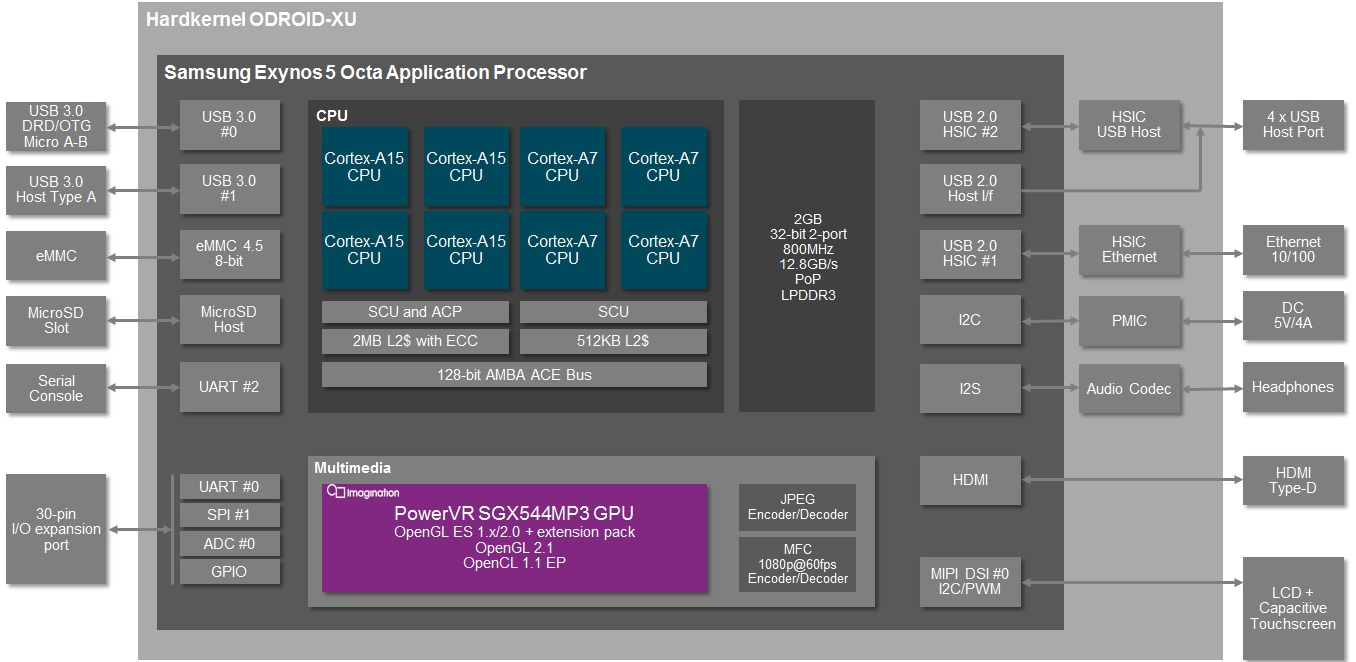
\includegraphics[width=0.9\linewidth]{Figures/Hardkernel-ODROID-XU-block_diagram.jpg}
\caption{Hardkernel Odroid-XU block diagram}
\label{odroid-xu}
\end{figure}

\section{Implementation}
\lstset{language=C++}

As stated before, on the Odroid-XU board only one of the two clusters can run at the same time. Since our application is heavy, we choose the A15 cluster, which includes four cores and is the most performant cluster. This is done trough the following command:
\begin{lstlisting}[frame=single]  % Start your code-block

echo performance > /sys/devices/system/cpu/cpu0/cpufreq/scaling_governor
\end{lstlisting}
which basically activates the \verb+performance+ governor as the controller for the big.LITTLE switching mechanism.
Then, having written a sequential implementation of our algorithm using the OpenCV library\footnote{This is joint work with Francesco Paci.}, we compile it using \verb+gcc+ with the following options:
\begin{lstlisting}[frame=single]  % Start your code-block

-g -mfpu=neon-vfpv4 -ftree-vectorize -mfloat-abi=hard -mtune=cortex-a15 -marm
\end{lstlisting}

The \verb+-g+ flag tells the compiler to produce debugging information in the operating system's native format, \verb+-mfpu=neon+  specifies what floating-point hardware (or hardware emulation) is available on the target, \verb+-ftree-vectorize+ enables the auto-vectorizer (which will try to use SIMD instructions, when possible), \verb+-mfloat-abi=hard+ allows generation of floating-point instructions and uses FPU-specific calling conventions, and \verb+-mtune=cortex-a15+ tunes the performance of the compiler for the A15 target.

\subsection{OpenMP and Neon Intrisics}
This first sequential version runs at 4.3 frames/s on $160\times 120$ frames, and needs 234 ms to elaborate each frame. The main bottleneck of this implementation is the multi-scale Farneback's optical flow, which requires 141 ms for each frame to run. Farneback's algorithm is executed two times for each frame, since the optical flow is calculated both on the original frame on the warped one, so we use OpenMP to run these two executions simultaneously on two different threads. Then, we use Neon intrinsics in order to exploit the SIMD capabilities of our CPU and thus gain a better performance on each thread.

A complete explanation of the optimizations made is beyond the purpose of this chapter, but, as an example, let's consider this for loop, which is responsible of 51 of the 234 ms:
\begin{lstlisting}[frame=single]  % Start your code-block

for( ; x < width*5; x++ ) {
	float s0 = srow[m][x]*kernel[0];
	for( i = 1; i <= m; i++ )
		s0 += (srow[m+i][x] + srow[m-i][x])*kernel[i];
	vsum[x] = s0;
}
\end{lstlisting}

Once optimized with Neon SIMD, the previous code becomes:
\begin{lstlisting}[frame=single]  % Start your code-block

int xstart = x;
float kernelext0[4];
fill_n(kernelext0,4,kernel[0]);
for( ; x < width*5-4; x+=4 ) {
           vst1q_f32(vsum+x, vmulq_f32(vld1q_f32(srow[m]+x),
		vld1q_f32(kernelext0)));
}
float a[width*5];
float kernelext[4];
for( i = 1; i <= m; i++ ) {
	fill_n(kernelext, 4, kernel[i]);
           for (x=xstart; x<width*5-4; x+=4) {
                        vst1q_f32(a+x, vaddq_f32(vld1q_f32(srow[m+i]+x), 
			vld1q_f32(srow[m-i]+x)));
                        vst1q_f32(vsum+x, vmlaq_f32(vld1q_f32(vsum+x), 
			vld1q_f32(a+x), vld1q_f32(kernelext)));
           }
}
\end{lstlisting}
As can be seen, the two for loops have been inverted and four floats are processed at each iteration. The new code block takes only 20 ms to run. 

\subsection{Further optimizations}
Having included several OpenMP/SIMD optimizations, our code runs at 7.1 frames/s on the A15 cluster, still not enough for real-time. Moreover, our algorithm needs an high frame rate in order to compute significant trajectories. Being the Farneback's algorithm our main bottleneck, we could turn our attention to the PowerVR GPU embedded into the Odroid board. Unfortunately, Hardkernel has not yet released an Ubuntu kernel that supports the PowerVR GPU\footnote{see: \url{http://forum.odroid.com/viewtopic.php?f=61&t=2236}.}, so the only way we have to increase speed is to further reduce the frame size and keep only one level of the spatial pyramid. Having reduce the frame size to $113\times 85$


... the Farneback's optical flow\footnote{\url{https://github.com/Itseez/opencv/blob/9aa4410509fcc60dfabb78c14a96ed5153ee117e/modules/ocl/src/opencl/optical_flow_farneback.cl}} is included in the C++ code.


\section{Some applications}
\subsection{Ego-Vision Jacket}
\subsection{...}
